\documentclass[crop,tikz]{standalone}
\usepackage{tikz}
\usetikzlibrary{calc}
\usetikzlibrary{positioning}
\begin{document}
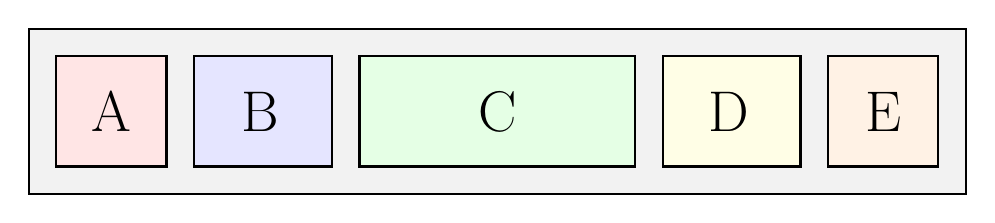
\begin{tikzpicture}[scale=0.07,rotate=0]
		
	%Frame
	\draw[thick, draw=black, fill=gray!10] (0,0) rectangle (170,30);

	%Segments
	%A
	\draw[thick, draw=black, fill=red!10] (5,5) rectangle (25,25);
	\node at (15,15) {\huge A};

	%B
	\draw[thick, draw=black, fill=blue!10] (30,5) rectangle (55,25);
	\node at (42,15) {\huge B};
	
	%C
	\draw[thick, draw=black, fill=green!10] (60,5) rectangle (110,25);
	\node at (85,15) {\huge C};

	%D
	\draw[thick, draw=black, fill=yellow!10] (115,5) rectangle (140,25);
	\node at (127,15) {\huge D};

	%E
	\draw[thick, draw=black, fill=orange!10] (145,5) rectangle (165,25);
	\node at (155,15) {\huge E};
	
\end{tikzpicture}
\end{document}